\chapter{Breezy Project: a DOTA 2 competition}
\label{chap:dota}

During the first month of my internship I teamed up with my supervisor \href{https://www.linkedin.com/in/dennis-g-wilson/}{\color{blue}{Assoc. Prof. Dennis Wilson}} and my fellow Research Intern \href{https://www.linkedin.com/in/lucashervier/}{\color{blue}{Lucas Hervier}} to participate in an Evolutionary Reinforcement Learning competition held as part of the international Genetic and Evolutionary Computation Conference, known as GECCO 2020, on the DOTA 2 video game.

\section{Context}
In 2018 the video game industry generated sales of more than US\$130 billion, reaching around 2 billion players around the world. Because video games can provide complex tasks necessitating short- and long-term planning in a controlled environment with no risks to humans \cite{Games_AI}, they also provide an excellent test-bed for Artificial Intelligence (AI) systems. Multiple learning agents have been tested on the Arcade Learning Environment based on Atari 2600 games \cite{Atari}, including Reinforcement Learning (RL) techniques like Deep Q Networks \cite{DQN} and Agent57 \cite{agent57}. Other games such as StarCraft, DOTA2, Mario, or Doom, have also been extensively used as machine learning benchmarks.

Since the reward in games is often sparse, making the learning signal weak, gradient-based methods might struggle for the optimization of neural network parameters. Evolutionary Strategies (ES), which estimate the gradient of the objective function without needing an explicit gradient definition, have been used to optimize Deep Convolutional Neural Networks \cite{CMAES_DL}, and the evolution of synaptic weights have been demonstrated to be competitive with deep RL methods\cite{deep_neuroevo}.\\

In this context, \href{https://web.cs.dal.ca/~dota2/?page_id=353}{\color{blue} {Project Breezy}} is a competition created by Robert Smith and Malcolm Heywood from Dalhousie University to develop a \href{https://store.steampowered.com/app/570/Dota_2/}{\color{blue}{DOTA 2}}-playing bot evolved with evolutionary algorithms, in a 1-versus-1 symmetrical match-up. 

We entered this competition as an opportunity to try and test neuroevolution algorithms on a complex real-time game, and as a step towards the development of a comprehensive benchmark of Evolutionary Reinforcement Learning algorithms.

\section{DOTA 2 as a RL environment}
\subsection{The game}

\href{https://en.wikipedia.org/wiki/Dota_2}{\color{blue}{Dota 2}} is the sequel of Defense of the Ancients (DotA), a community-created game mod for Warcraft III that popularised the Multiplayer Online Battle in Arena (\href{https://en.wikipedia.org/wiki/Multiplayer_online_battle_arena}{\color{blue}{MOBA}}) video game genre. In Dota 2, 2 teams (called "Radiant" and "Dire") of 5 players compete to destroy the main structure of the enemy's base (the "Ancient") in a real-time strategy game, each player controlling one of the 119 possible characters (the "heroes").

\begin{figure}[H]
 \centering
 \captionsetup{justification=centering, margin=0.5cm}
 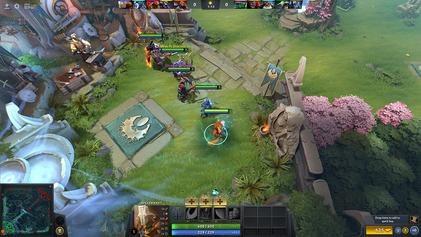
\includegraphics[width=8cm]{images/Dota_2_Gameplay_Aug_2017.jpg}
\caption{A game of Dota 2 in progress, showing the Radiant team inside their base at the beginning of a match (\href{https://en.wikipedia.org/wiki/Dota_2}{\color{blue}{Source}})}
 \label{fig:dota-2-game}
\end{figure}

The game takes place on a square map (cf fig. \ref{fig:dota-2-map}) which contains both team-controlled buildings (e.g. towers, barracks) that the other team can attack, and neutral objectives (e.g. Roshan). Team bases are situated in the bottom-left and top-right corners respectively, with 3 lanes joining them called the top (through the top-left corner), the middle (diagonally), and the bottom (through bottom-right corner) lane, each guarded by towers and around which most early gameplay happens. Creeps are basic AI-controlled units that periodically spawn for each team at the barracks and walk down the lane to help destroy enemy buildings. Dealing the last hit ("last hitting") an enemy creep is rewarded with money, which allows to buy items influencing the player's hero strengths. Last hitting a creep of the same team allows to deny them from the enemy. 

\begin{figure}[H]
 \centering
 \captionsetup{justification=centering, margin=0.5cm}
 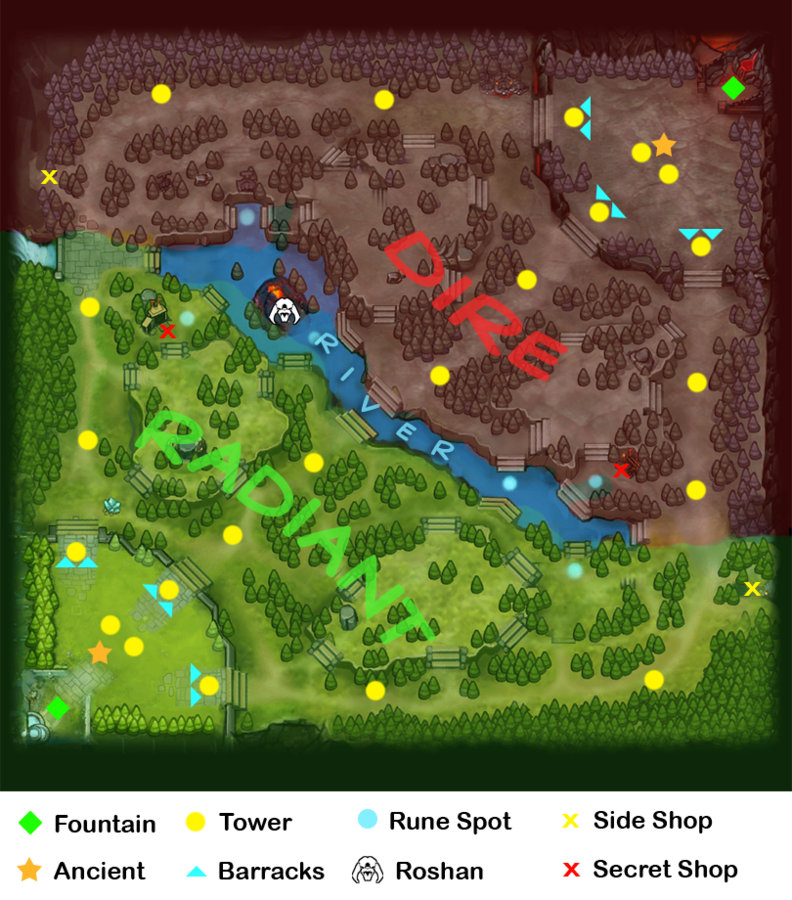
\includegraphics[width=8cm]{images/dota-map.png}
\caption{Labelled Dota 2 map as of version 7.20 (\href{https://dota2.gamepedia.com/Map}{\color{blue}{Source}})}
 \label{fig:dota-2-map}
\end{figure}

The 1v1 game mode opposes only 1 player in each team, and can be won by either killing the enemy twice, or destroying the first enemy tower on the middle lane. \\
The game mode used for this competition additionally fixes the heroes to be \href{https://dota2.gamepedia.com/Shadow_Fiend}{\color{blue}{Shadow Fiend}} for both players, for balancing purposes.

\subsection{Project Breezy}
\href{https://web.cs.dal.ca/~dota2/?page_id=353}{\color{blue} {Project Breezy}} provides software to enable communication with the Dota 2 game by opening a server communicating with the game instance. The agent, through a Python server, interacts with the Breezy server, getting the game state and sending action orders. The game state contains 310 features such as health points, hero position, creeps positions, or spell cooldowns. 29 actions are available, including movementS, spell casting, or attacking.

\subsection{Challenges}
Evolving Neural Networks to play Dota 2 is subject to multiple constraints:
\begin{itemize}
    \item \textbf{Processing time}: Since DOTA 2 is a real-time game, the generated neural networks needs to be fast to evaluate at each step.
    \item \textbf{Evaluation time}: Even sped up, evaluating a policy requires running a full game in a simulator, hence the number of evaluations is a strong limiting factor.
    \item \textbf{Network size}: Due to the large size of the game state provided by the Breezy server and the hight number of possible actions, generated neural networks might require large architectures, hence increasing computation time and problem dimensionality.
    \item\textbf{Network complexity}: Since Dota 2 requires both short- and long-term planning, more complex architectures might be required 
    \item \textbf{Fitness sparsity}: Since the fitness used rewards dealing damage and last hitting, many behaviors that do not get close enough to the enemy have the same fitness, hence information about the quality of an individual is rare and requires already advanced policies
\end{itemize}

\section{Our approach}

\subsection{Problem Modeling}
\label{sec:representation choice}

\subsubsection{Fitness Function}
In order to win a 1v1, a player needs to kill the opponent twice or to take his first mid tower. Consequently, we took into account the number of times we killed the opponent champion and the opponent tower health in the individual evaluation. Moreover, to succeed in one of those two tasks one would also need good laning skills. Therefore, we also took into account the amount of gold collected (\textit{net worth}), the number of last hits, and the number of denies. We also punished being killed and behaviors causing an early stopping.

\begin{minipage}{\linewidth}
The final fitness function is hence as follows:

\begin{equation*}
\label{eq:fitness}
\begin{minipage}{0.45\textwidth}
% \begin{multline*}
\begin{split}
 fitness & = netWorth + 100*lastHits + 100*denies\\
         & + 2000*ratioTowerHealth + 1000*nbKill\\
         & - 250*nbDeath - 500*earlyStop\\
 \end{split}
% \end{multline*}
\end{minipage}
\end{equation*}
\end{minipage}


\subsubsection{Behavior Space}
Our goal with a Quality-Diversity approach was to observe individuals with highly diverse behaviors to increase our chances of finding interesting ones. Therefore, we needed a characterization of the behavior space to differenciate playstyles. 
We described the behavior in a discretized 2-dimensional space featuring the \textit{total damage made to the opponent champion} and the \textit{percentage of the opponent tower health taken} as axes, since the objective was either to kill the opponent champion or to take his tower. 

\subsection{Reducing the evaluation cost}
We quickly realized that one of the main difficulty of this challenge was to deal with the evaluation cost of the fitness. Indeed, in order to evaluate an agent we need him to play a full DOTA2 game which can take up to several minutes in real time, even with a tenfold speeding. Since Evolutionnary Algorithms (EAs) require a large number of function evaluations, we had to find a way to cope with this issue. 

\subsubsection{Early stopping}
A simple but efficient way of reducing the evaluation time was to use an Early Stopping mechanism. We decided to stop the evaluation of an agent if he did not kill a creep after 5min of DOTA time. This functionality reduced the time loss due to static individual, and the evaluation length of "coward individuals" avoiding fights.

\subsubsection{Neural-base simulator}
Since an evaluation is time consuming, we developped a \href{https://github.com/TemplierPaul/Dota_Simulator}{\textbf{Dota Simulator}} to predict game state evolutions from previous state and chosen action, using a neural network based on the UNet \cite{UNet} architecture which we trained on random play. It was used in the offsprings generation phase:
\begin{itemize}
    \item offsprings are generated for 10 times the size of population 
    \item 100 game steps are simulated for each offspring, and the actions stored
    \item the actions taken by each individual are used to select the \textit{population size} most unique offsprings based on behavior
    \item those individuals are added to the new population and evaluated in the real game
\end{itemize}
By doing so we are seeing much more mutation and/or crossover. Moreover, taking the individuals the more distant from each other increases our chances to cover the behavior space.

\subsection{Algorithms}
We chose to train both CGP Individuals  \cite{CGP} and NEAT Individuals \cite{NEAT_1}, as defined in the respective papers, in a MAP-Elites algorithm. They were implemented with \href{https://github.com/d9w/CartesianGeneticProgramming.jl}{\textbf{CartesianGeneticProgramming.jl}} for the CGP agent, and a custom NEAT agent developed at \href{https://github.com/d9w/NEAT.jl}{\textbf{NEAT.jl}} for this challenge.

As we believed the best way to find interesting individuals, either with NEAT or with CGP, was to explore the behavorial space, we based the exploration on the \textbf{Illuminating search spaces by mapping elites} \cite{MapElites} paper. 

\section{Results}

Results were announced at GECCO 2020 on July 12\textsuperscript{th} by the organizers. \\
9 teams had registered to the competition, but only 2 -including us- provided code to be evaluated, among which we ranked first. \\

\begin{figure}[H]
\centering
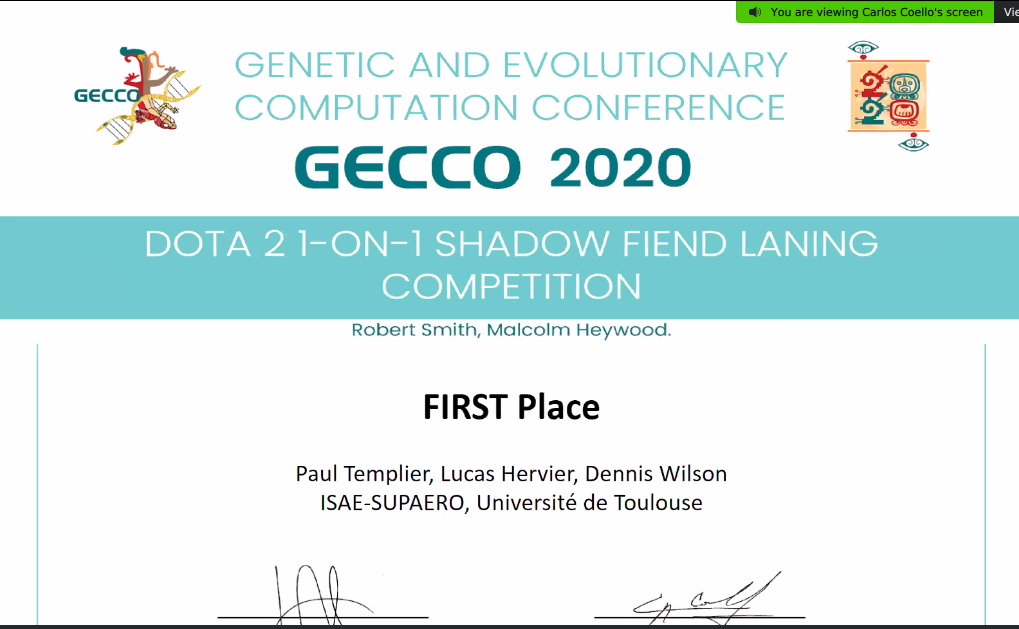
\includegraphics[width=12cm]{images/breezy-win.png}
\caption{Competition results announcement at GECCO 2020}
\end{figure}

%%% Local Variables: 
%%% mode: latex
%%% TeX-master: "isae-report-template"
%%% End: 